\documentclass[11pt,a4paper]{article}
\usepackage{{../../paquete}}
\usepackage{{../../estilos}}
\graphicspath{{../Figuras}}
%BEGIN_FOLD Comandos
\newcommand{\nombreMateria}{Mecánica de Fluidos y Máquinas Fluidodinámicas}
\newcommand{\materia}{\textit{\nombreMateria}}
%END_FOLD
\fancyhead[L]{\textsc{\nombreMateria}}

\begin{document}
%	\ProvidesPackage{portada}

\usepackage{tikz}
\usepackage{setspace}
\definecolor{maincolor}{HTML}{213250}

\makeatletter
\renewcommand{\maketitle}{
	\begin{titlepage}\centering
		\begin{tikzpicture}[remember picture, overlay]
			\draw[line width=60pt, color=maincolor] 
			([xshift=1cm, yshift=-1cm]current page.north west) 
			rectangle 
			([xshift=-1cm, yshift=1cm]current page.south east);
		\end{tikzpicture}
		\vfill
		
\includegraphics[width=4cm]{recursos/logo}\\[5pt]
		{\Large \textsc{Universidad Tecnológica Nacional}\\[5pt]
			Facultad Regional Reconquista\\[5pt]
			Ingeniería Electromecánica}\\[3cm]
		
		\begin{minipage}{.7\linewidth}
			\centering
			\setstretch{.9}
			{\Huge\textbf{\@title}\\[5pt]
				\LARGE \emph{Apunte de Cátedra} \par}
			\vspace{3cm}
		\end{minipage}
		\vfill
		{\@author\\[5pt]
			\large \@date}
		\vfill
	\end{titlepage}
}
\makeatother
 para que no ande cargando a cada rato cuando compilo sino tarda
	\pagestyle{fancy}
	\section{Conceptos generales}

\subsection{Definición de un fluido}
Un fluido es una sustancia que siempre se deforma continuamente cuando se somete a un esfuerzo cortante, sin importar qué tan pequeño sea dicho esfuerzo.\\

Tiene \textbf{propiedades} que lo caracterizan y definen el estado en el que se encuentra, pudiendo determinar su comportamiento. Algunas de estas propiedades son: \\
\begin{center}
	\begin{tabular} {r l}
		Densidad & $\rho = \dfrac{m}{V} \;[kg/m^3]$ \\
		Viscosidad & $\mu \;[kg/m s]$ \\
		Peso & $P \;[kgf] [N]$\\
		Peso específico & $\gamma \;[kgf/m^3]$ \\
		Temperatura & $T \;[°C]$ \\
	\end{tabular}
\end{center}

A fines de simplificar cálculos, consideramos la densidad de un fluido constante.

También consideramos la estructura molecular de los fluidos como \emph{continuo}, esto quiere decir que las propiedades de este varían en forma continua a lo largo de su estructura o se mantienen constantes.


\subsection{Ecuación de Newton para los fluidos}
Para obtener la ecuación de newton para los fluidos, se plantea un sistema en el que un fluido se entra entre dos placas paralelas separadas por una cierta distancia, como se muestra en la figura \ref{fig:fluido-placas-paralelas}. La placa inferior es fija y a la superior se le aplica una fuerza $F$ lo que produce un esfuerzo cortante en el fluido, y a su vez establece una velocidad en la placa superior.

Si la fuerza $F$, por más pequeña que sea, hace que la placa se mueva permanentemente, entonces la sustancia es un fluido.

\begin{figure}[H]
	\centering
	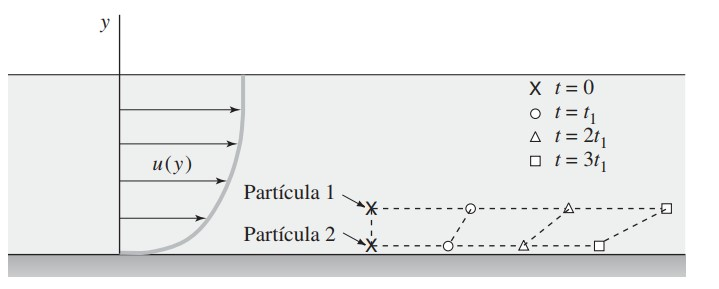
\includegraphics[width = .8\linewidth]{U1-cortante3}
	\caption{Movimiento relativo de dos partículas de fluido en presencia de esfuerzos cortantes}
	\label{fig:fluido-placas-paralelas}
 \end{figure}

Manteniendo ciertas cantidades constantes, como la viscosidad $\mu$ del fluido, el area de las placas, la distancia entre ellas y la velocidad de la placa superior, se llega a una expresión que relaciona la fuerza aplicada con los parámetros mencionados:
\begin{equation}
	F = \mu \dfrac{A \cdot U}{y}
	\label{eq:fuerza}
\end{equation}

Considerando que el esfuerzo se calcula como la fuerza aplicada en un área:

\begin{equation*}
	\tau = \dfrac{F}{A}
	\label{eq:esfuerzo}
\end{equation*}

y reemplazando a la fuerza $F$ por la expresión \ref{eq:fuerza} se llega a la ecuación para determinar el esfuerzo cortante en función de la viscosidad, la velocidad del fluido y la altura:

\begin{equation}
	\tau = \mu \dfrac{U}{y} \hspace{.3cm};\hspace{.3cm} \tau = \mu \dfrac{du}{dy}
\end{equation}

El término $\dfrac{du}{dy}$ es un gradiente de velocidad y puede ser interpretada como una \textbf{velocidad de deformación}.\\ 


A partir de esta definición, los fluidos se pueden clasificar como \textit{newtonianos} o \textit{no newtonianos}.

\subsubsection{Fluidos newtonianos}

Los fluidos newtonianos son aquellos fluidos donde su viscosidad es constante, es decir, la relación entre el esfuerzo cortante y de velocidad de deformación es lineal, como se muestra en la figura \ref{diag:fluido-newtoniano}.



\begin{figure}[H]
	\centering
	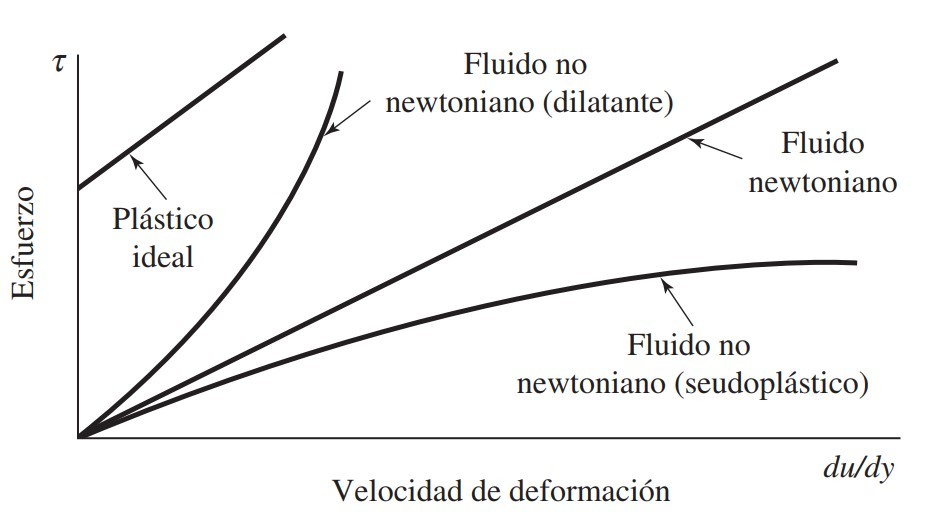
\includegraphics[width= .7\linewidth]{U1-tipo-fluido}
	\caption{Fluidos newtonianos y no newtonianos}
	\label{diag:fluido-newtoniano}
\end{figure}

\subsubsection{Fluidos ideales}

Un fluido ideal se considera cuando su viscosidad es nula, por lo tanto el esfuerzo cortante requerido será nulo sin importar su movimiento.

En la figura \ref{diag:fluido-newtoniano} un fluido ideal se representaría como una recta vertical que atraviesa el origen de coordenadas.



\subsection{Viscosidad}
\subsubsection{Viscosidad absoluta o dinámica $\mu$}
La viscosidad es una propiedad propia del fluido e indica el grado de resistencia a los esfuerzos cortantes.

En los gases, la viscosidad absoluta incrementa con la temperatura, en cambio, en los líquidos disminuye junto con esta. 

En un líquido, esto se debe directamente a la cohesión entre las moléculas de la sustancia. Esta disminuye cuando aumenta la temperatura. En cambio en gases, la viscosidad se debe por el movimiento aleatorio de las moléculas, y éste aumenta con la temperatura.

\subsubsection{Viscosidad cinemática $v$}

Es la relación entre la viscosidad absoluta y la densidad de la sustancia
\begin{equation}
	v = \dfrac{\mu}{\rho}
\end{equation}

\subsection{Compresibilidad y tensión superficial}
\subsubsection{Compresibilidad}
La compresibilidad es la capacidad de un fluido de disminuir su volumen bajo la aplicación de una presión. Los gases son altamente compresibles mientra que los líquidos, muy poco. 

En la materia \materia se trabaja con fluidos ideales no compresibles, es decir, de viscosidad cero.\\

\subsubsection{Tensión superficial}

El fenómeno de tensión superficial se debe a las fuerzas de cohesión y adhesión entre las partículas. Sobre la superficie del liquido las fuerzas cohesivas desde abajo exceden a las fuerzas adhesivas desde el gas localizado por encima del fluido (figura \ref{fuerzas_cohesivas_adhesivas}), dando como resultado una tensión superficial.

\begin{figure}[h]
	\centering
	\begin{subfigure}[b]{.45\linewidth}
		\centering
		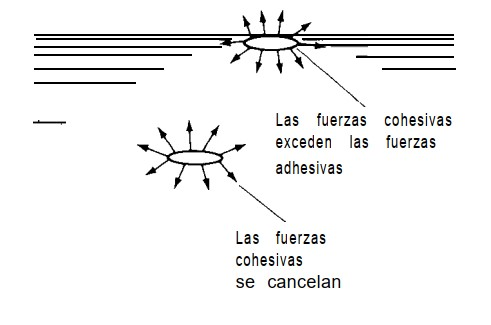
\includegraphics[width = .7\linewidth]{U2-fuerzas}
		\caption{Fuerzas cohesivas y adhesivas}
		\label{fuerzas_cohesivas_adhesivas}
	\end{subfigure}
	\begin{subfigure}[b]{.45\linewidth}
		\centering
		\begin{subfigure}[b]{.45\linewidth}
			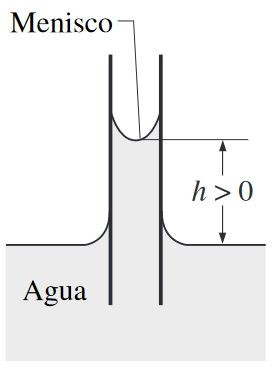
\includegraphics[width = .9\linewidth]{U1-efecto-capilar-agua}
			\caption{}
			\label{fig:capilaridad-agua}
		\end{subfigure}
		\begin{subfigure}[b]{.45\linewidth}
			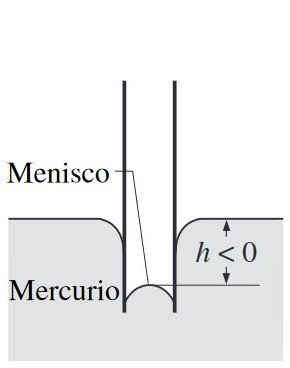
\includegraphics[width = .9\linewidth]{U1-efecto-capilar-mercurio}
			\caption{}
			\label{fig:capilaridad-mercurio}
		\end{subfigure}
	\end{subfigure}
	\caption{Tensión superficial}
\end{figure}

En el caso de un líquido que se encuentra en contacto con un sólido, si la adhesión del líquido con el sólido es mayor que la cohesión en el líquido mismo, entonces éste \emph{subirá} dentro del tubo y formará con el sólido un menisco curvado hacia arriba, como muestra la figura \ref{fig:capilaridad-agua}. Puede pasar también que las fuerzas de adhesión sean menores que las de cohesión y entonces el menisco estará curvado hacia abajo, como el caso del mercurio y el vidrio de la figura \ref{fig:capilaridad-mercurio}.\\ %Ver para agregar la figura del mercurio, entoces queda más copado si se puede ver el efecto.

Podemos calcular la altura h que se desplaza el fluido igualando la componente vertical de la fuerza de tensión superficial (que actúa en la dirección $\theta$) con el peso de la columna de fluido, como:
%Agregar una imagen del esquema, si es que hay una, entonces no queda al aire el planteo

\begin{equation*}
	\sigma \pi \cos \beta = \gamma \dfrac{\pi D^2}{4} h
\end{equation*}
\begin{equation}
	h = \dfrac{4 \sigma \cos \beta}{\gamma D}
\end{equation}

donde $\sigma$ es la tensión superficial.

\subsection{Presión de vapor}
Cuando un liquido se evapora, las moléculas escapan desde la superficie líquida.  Si el espacio por encima del líquido se encuentra confinado, el equilibrio se logrará cuando el número de moléculas de vapor que se condensan es igual al número de moléculas que escapan de la superficie. La presión resultante de las moléculas de vapor se conoce como \emph{presión de vapor} y es directamente proporcional a la temperatura. Cuando la presión por encima del líquido iguala a la presión de vapor de este, se produce la ebullición. \\

En flujos líquidos, pueden crearse condiciones que lleven la presión por debajo de la presión de vapor del líquido. Cuando ocurre esto se forman burbujas localmente, fenómeno llamado \emph{cavitación}.




	\section{Estática de los fluidos}

La \textbf{estática de fluidos} es el estudio de fluidos en los que no hay movimiento relativo entre sus partículas. Si no hay movimiento relativo, no existen gradientes de velocidad $\sfrac{du}{dy}$, por lo cual los esfuerzos cortantes serán nulos. El único esfuerzo que existe es un esfuerzo normal, la presión, de modo que ésta tiene la mayor importancia en este estudio.


\subsection{Presión en el seno de los fluidos}%Ver mejor este título

\subsubsection{Presión en un punto}

La presión en un punto de un fluido es constante, es decir, \textsl{la presión es una función escalar y no depende de la dirección normal del área}. Actúa igualmente en todas las direcciones.

\begin{equation}
	p_x = p_y = p_z = p
\end{equation}

%Esta imagen estaba por la demostracion pero me dio paja escribir todo, si quieren saquenla o dejenla, para que se entienda a qué van las p que están arriba...o sea, px py pz
\begin{figure}[H]
	\centering
	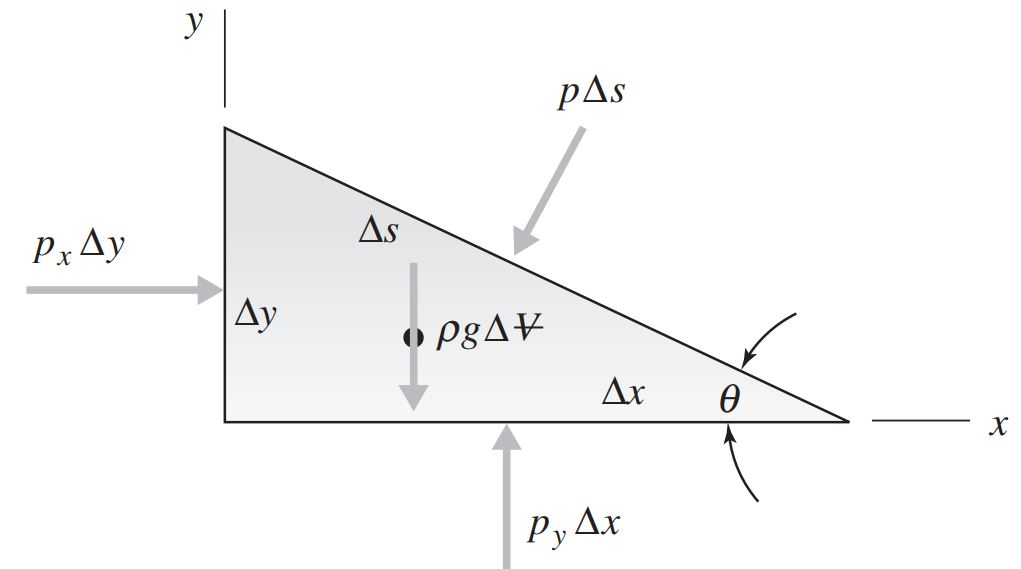
\includegraphics[width = .5 \linewidth]{fluido-infinitesimal}
	\caption{Presión en un punto en un fluido.}
	\label{fig:elemento-infinitesimal}
\end{figure}

\subsubsection{Variación de presión}

%Para determinar la variación de presión de fluidos en reposo, se considera el elemento infinitesimal que se ilustra en la figura \ref{fig:elem-infinitesimal}.
%
%\begin{figure}[H] 
%	\centering
%	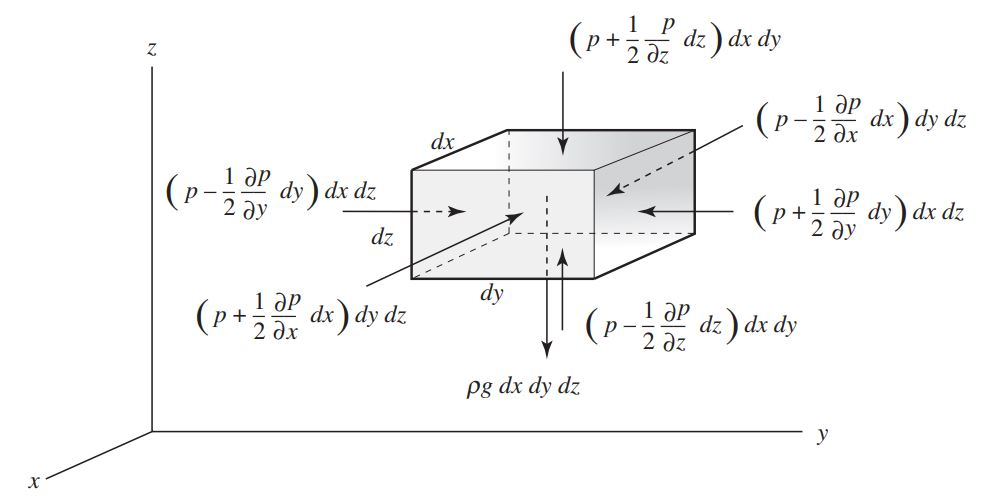
\includegraphics[width = .8\linewidth]{elemento-infinitesimal}
%	\caption{Fuerzas que actúan sobre un elemento infinitesimal de fluido.}
%	\label{fig:elem-infinitesimal}
%\end{figure}
%
%Las presiones en cada uno de los lados se pueden expresar utilizando la \textsl{regla de la cadena} del cálculo infinitesimal con $p\left(x,y,z\right)$:
%
%\begin{equation*}
%	dp = \dfrac{\partial p}{\partial x} dx + \dfrac{\partial p}{\partial y} dy + \dfrac{\partial p}{\partial z} dz
%\end{equation*}
%
%Si nos movemos una distancia $\dfrac{dx}{2}$, la presión será:
%
%\begin{equation*}
%	p\left(x + \dfrac{dx}{2},y,z\right) = p(x,y,z) + \dfrac{\partial p}{\partial x} \dfrac{dx}{2}
%\end{equation*}
%
%Considerando a la Ley de Newton en forma vectorial para un sistema de masa constante como la sumatoria de las fuerzas igualadas a la aceleración por su masa, se llega a tres ecuaciones de componentes:
%
%\begin{align*}
%	-\dfrac{\partial p}{\partial x}\ dx\ dy\ dz & = \rho a_x\ dx\ dy\ dz\\
%	-\dfrac{\partial p}{\partial y}\ dx\ dy\ dz & = \rho a_y\ dx\ dy\ dz\\
%	-\dfrac{\partial p}{\partial z}\ dx\ dy\ dz & = \rho (a_z+g)\ dx\ dy\ dz\\
%\end{align*}

Para determinar la variación de presión de fluidos se utiliza la ecuación \ref{eq:variacion-de-presion} que representa el diferencial de presión en cualquier dirección. 

\begin{equation}
	dp = -\rho a_x dx -\rho a_y dy -\rho (a_z + g) dz
	\label{eq:variacion-de-presion}
\end{equation}

En la estática de fluidos se trabajan con fluidos en reposo, es decir, que no tienen aceleración además de la que experimentan con la aceleración de la gravedad ($a_x = a_y = a_z = 0$).\\


Entonces, para dichos fluidos se llega a la \textbf{ecuación fundamental de la hidrostática}, donde la presión varía en la dirección vertical:

\begin{equation}
	\dfrac{dp}{dz}= - \gamma = - \rho\ g
	\label{eq:fundamental}
\end{equation}

Tambien, tenemos que tener en cuenta que $dp$ se incrementa cuando $dz$ disminuye; esto es, la presión \textbf{aumenta} cuando nos movemos \textbf{hacia abajo} y disminuye cuando es hacia arriba.\\

Si se integra la ecuación \ref{eq:fundamental} se llega a:

\begin{equation}
	P_1 - P_2 = \gamma (z_2 - z_1)
	\label{eq:fundamental-integrada}
\end{equation}\\


Supongamos ahora que se tiene un fluido contenido en un vaso de precipitado como se ilustra en la figura \ref{fig:precipitado}. 

\begin{figure}[H]
	\centering
	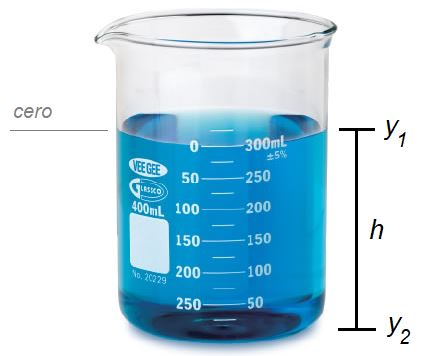
\includegraphics[width = .3\linewidth]{vaso-de-precipitado}
	\caption{Presión en un fluido en reposo}
	\label{fig:precipitado}
\end{figure}

Al estar en contacto con el aire, la presión en el punto 2 será la atmosférica $P_{atm}$, y la ecuación \ref{eq:fundamental-integrada} quedará de la siguiente manera:

%Falta...
\begin{tikzpicture}
	% Ejes cartesianos
	\draw[gray, thick] (0, 0) -- (4, 0) node[right] {$x$};
	\draw[gray, thick] (0,0) -- (0, 4.5) node[right] {$y$};
	
	% Estilo de la función lineal decreciente
	\tikzset{funcion/.style={black, thick}}
	
	% Función lineal decreciente
	\draw[funcion] (1.01325, 4) -- (1.01325+1, 0) node[right] {$P_1(h) = P_{atm} + \gamma\ h$};

	
\end{tikzpicture}



\begin{equation}
	P_1 - P_{atm} = \gamma (z_2 - z_1)
\end{equation}


A la diferencia $P_1 - P_{atm}$ se la denomina como \textbf{presión hidrostática} o manométrica.\\



Si se despeja la presión $P_1$ se llega a la expresión para el \textbf{Segundo Principio de Pascal}:

\begin{equation}
	P_1 = P_{atm} + \gamma h
\end{equation}

\subsection{Manómetros} %Ver este también
Los manómetros son instrumentos que usan columnas de líquidos para medir presiones. Estudiaremos tres tipos, pero todos se basan en la ecuación fundamental de la hidrostática:

\subsubsection{Manómetro de tubo U}
Para medir presiones relativamente pequeñas, usamos un manómetro como se ve en la figura \ref{fig:manometro-u}. Si trazamos una linea horizontal imaginaria que pase por 1, la presión en ambos lados del manómetro será igual. Entonces
\begin{gather}
	P_{1} = P_{1'} \\
	P_{1} = P_{2} + \gamma \, h = P_{atm} + \gamma \, h\\
\end{gather}
Donde $\gamma$ es el peso específico del fluido que se utilize

\begin{figure}[h]
	\centering
	\begin{subfigure}[b]{.45\linewidth}
		\centering
		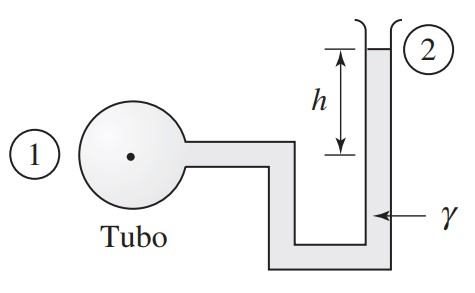
\includegraphics[width = .6\linewidth]{U2-manometro-U}
		\caption{Presiónes pequeñas}
		\label{fig:manometro-u}
	\end{subfigure}
	\begin{subfigure}[b]{.45\linewidth}
		\centering
		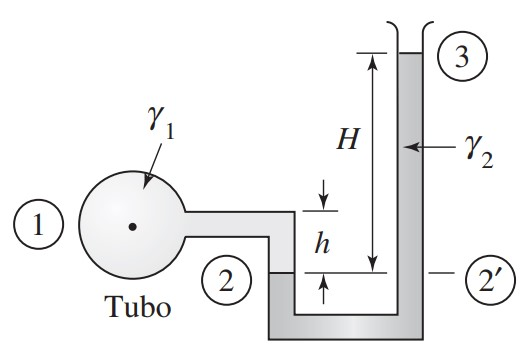
\includegraphics[width = .6\linewidth]{U2-manometro-U1}
		\caption{Presiónes grandes}
		\label{fig:manometro-u2}
	\end{subfigure}
	\caption{Manómetros de tubo en U}
\end{figure}

Cuando necesitemos medir presiones relativamente grandes usamos un manómetro como se ve en la figura \ref{fig:manometro-u2}. Siguiendo la misma metodología que el caso anterior, pero ahora existen dos fluidos no miscibles dentro del tubo.

\begin{gather}
	P_{2} = P_{2'}\\
	P_{1} + \gamma_{1} h = P_{atm} + \gamma_{2} H 
\end{gather}

\subsubsection{Micromanómetro}
Lo usamos para medir cambios de presión muy pequeños. Seguimos con el mismo principio que usamos anteriormente.
\begin{gather}
	P_{3}=P_{3'}\\
	P_{1} + \gamma_{1} (z_{1}-z_{2}) + \gamma_{2} (z_{2}-z_{3}) = P_{5} + \gamma_{2} (z_{5} - z_{4}) + \gamma_{3} (z_{4} - z_{3'})
\end{gather}
Observando que $z_{2}-z_{3} + h = z_{5} - z_{4} + H$
\begin{gather}
	P_{1} = \gamma_{1} (z_{2} - z_{1}) + \gamma_{2} (h- H) + \gamma_{3} \\
	P_{1} = \gamma_{1} (z_{2} - z_{1}) + \gamma_{2} h + (\gamma_{3} -\gamma_{2}) H
\end{gather}

\begin{figure}[h]
	\centering
	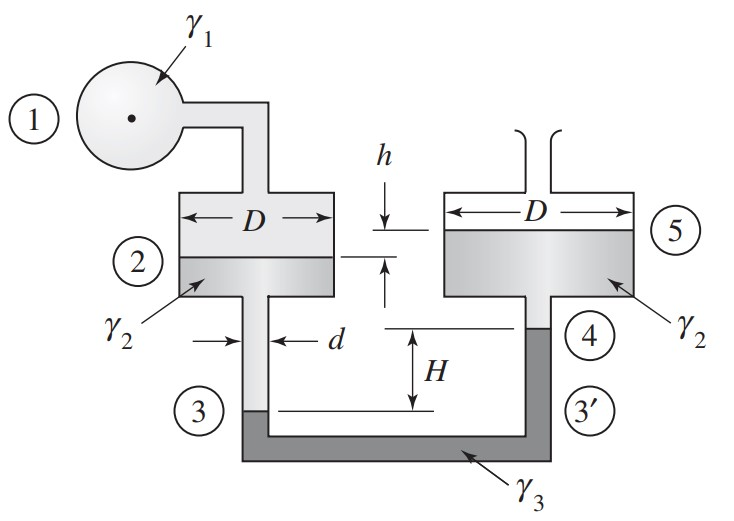
\includegraphics[width = .4\linewidth]{U2-micromanometro}
	\caption{Micromanómetro}
	\label{fig:micro}
\end{figure}
\subsubsection{Efecto de la fuerza superficial sobre un fluido confinado}
Si se ejerce una presión externa sobre una parte de la frontera de un fluido confinado, esta presión se transmite uniformemente a través de todo el fluido.
\\
Este principio explica el funcionamiento de gatos hidráulicos, prensas, frenos, y diversos mecanismos que transmiten fuerzas a través de un fluido.


\begin{figure}[h]	
	\centering
	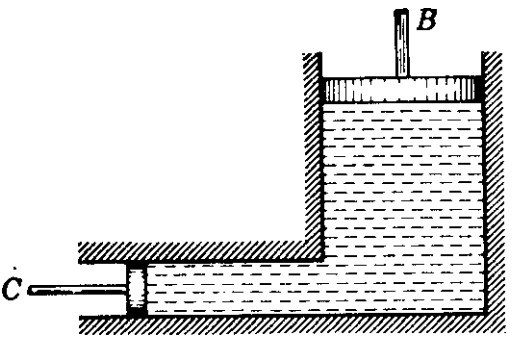
\includegraphics[width = .2\linewidth]{U2-gato-hidraulico}
	\caption{Gato hidráulico}
	\label{fig:gato}
\end{figure}

\begin{equation}
	\dfrac{F_{B}}{F_{C}} = \dfrac{\Delta P A_{B}}{\Delta P A_{C}} = \dfrac{A_{B}}{A_{C}}
\end{equation}


\subsection{Fuerzas sobre superficies}
\subsubsection{Planas}
Si sumergimos una placa plana, sobre ésta actuara una presión constante (sobre la superficie libre) y una presión causada por la gravedad que se incrementa uniformemente.
\begin{figure}[h]
	\centering
	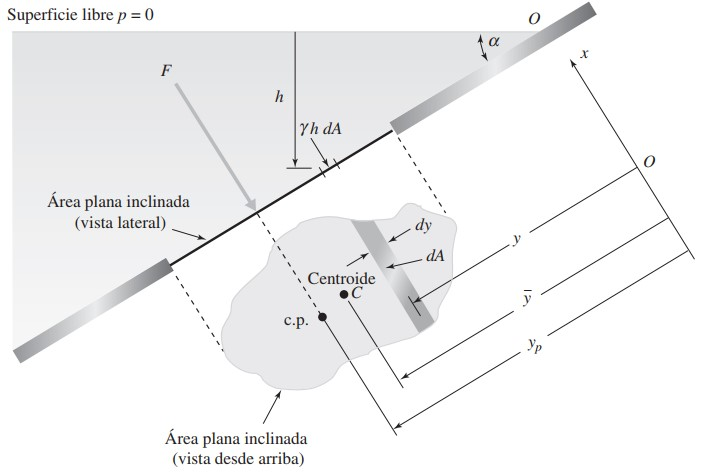
\includegraphics[width = .6\linewidth]{U2-sup-plana}
	\caption{Fuerza sobre área plana}
	\label{fig:sup-plana}
\end{figure}
Debido a que no puede existir esfuerzo cortante, esta fuerza debe ser perpendicular a la superficie sumergida. Observando la figura \ref{fig:sup-plana}, sobre el elemento \textbf{dA} actúa una presión constante. La magnitud de la fuerza sobre este elemento será $\gamma \, h \, dA$. Si integramos sobre el área completa de la placa
\begin{equation*}
	F = \int_{A} \gamma \ h \ dA = \int_{A} \gamma \ y \sin \theta \ dA =  \gamma \sin \theta \int_{A} y \ dA
\end{equation*}
La integral que queda es el primer momento de \emph{área} de la placa con respecto al eje \emph{x}; esto es equivalente a usar \textbf{$A \ \overline{y}$}, doonde $\overline{y}$ es la distancia al centroide de la superficie. Entonces la magnitud de la fuerza, teniendo en cuenta la presion en la superficie libre será:

\begin{equation}
	F =(P_{s} + \overline{y} \sin \theta \ \gamma) A
\end{equation}

Como la fuerza resultante no actúa en el centroide de la placa, para hallar la ubicación de esta igualamos la suma de los momentos de todas las fuerzas de presión que actúan sobre el área con el momento generado por la fuerza misma. Si la fuerza F actúa en el punto $(x_{p}, y_{p})$:

\begin{equation*}
	y_{p} F = \int_{A} y (P_{s} \overline{y} \sin \theta \ \gamma ) dA
\end{equation*}

Desarrollando llegamos a la siguiente ecuación:

\begin{equation}
	y_{p} = \overline{y} + \dfrac{\overline{I}_{x}}{A \overline{y}}
\end{equation}

Donde $\overline{I}_{x}$ es el momento de inercia centroidal de la placa respecto de $x$.
\\
De igual manera para hallar la coordenada $x_{p}$
\begin{equation*}
	x_{p} F = \int_{A} y (P_{s} \ \overline{y} \ \sin \ \theta \ \gamma ) dA
\end{equation*}
\begin{equation}
	x_{p} = \overline{x} + \dfrac{\overline{I}_{xy}}{A \overline{y}}
\end{equation}
Donde $\overline{I}_{xy}$ es el producto de inercia centroidal y $\overline{x}$ la distancia al eje $y$ centroidal.

\subsubsection{Curvas}
En este tipo de casos, no se utiliza un método directo para llegar al resultado, sino que se realiza un diagrama de cuerpo libre en el cual mediante integración se van determinando las fuerzas actuantes y ellas nos permitirán plantear las ecuaciones para los resultados.
\begin{figure}[h]
	\centering
	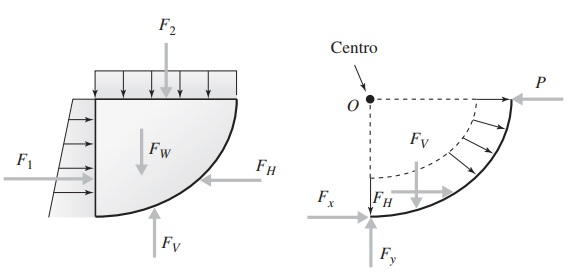
\includegraphics[width = .6\linewidth]{U2-curvas.jpg}
	\caption{Fuerza sobre superficies curvas}
	\label{fig:fuerz-sup-curv}
\end{figure}
Dicho DCL muestra las fuerzas debidas: al agua sobre la curva, $F_{1}$ y $F_{2}$ resultantes ubicadas debido a la distribución de las mismas y $F_{w}$ que es el agua del cuerpo inscripto en la figura. $F_{H}$ y $F_{V}$ son fuerzas que componen las reacciones y que mantienen el equilibrio en el sistema.\\
En este tipo de problemas la llave de la cuestión esta en hallar correctamente donde se encuentra esa fuerza $F_{w}$, conociendo ello solo basta plantear sumatoria de momentos respecto al vínculo de grado 2 de la compuerta.

\subsection{Cuerpos sumergidos}
\subsubsection{Empuje de flotación}
El \textbf{Princípio de Arquímedes} establece que la fuerza de flotación que aparece en un cuerpo sumergido es igual al peso del volumen de líquido desplazado.\\
También conocida como fuerza de boyamiento, resultante ejercida sobre un cuerpo por un fluido estático que se encuentra sumergido o flotando, esta fuerza siempre actúa verticalmente.
\begin{equation}
	F_{B}=\gamma V_{\text{líquido desplazado}}
	\label{ec:fuerz-boy}
\end{equation}
Donde esta fuerza de boyamiento actuará en el centroide del volumen desplazado. En líquidos compresibles no será asi ya que $\gamma$ depende de $z$.

\subsubsection{Estabilidad de flotación}
La \textbf{estabilidad vertical} la vemos cuando un objeto encuentra equilibrio entre el peso y la fuerza de boyamiento, cuando se lo quita del equilibrio (hundiendolo/removiendolo) aparecen fuerzas restauradoras que contribuyen a reponer el cuerpo nuevamente al equilibrio.\\
La \textbf{estabilidad rotacional} de un cuerpo sumergido.

\begin{figure}[!h]
	\centering
	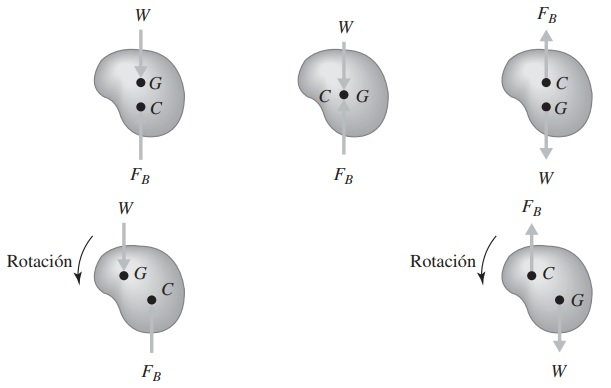
\includegraphics[width = .6\linewidth]{U2-estabilidad2.jpg}
	\caption{Estabilidad cuerpo sumergido}
	\label{fig:est-cuerp-sum}
\end{figure}


Para esto precisamos conocer el concepto de centro de flotabilidad $\textbf{C}$, que no es mas que el punto por el cual pasa la resultante de la fuerza de boyamiento.\\
Un análisis rápido nos que nos dará criterio para estabilidad depende de las posiciones relativas \textit{(cuál se encuentra arriba)}:\\
\begin{tabular}{p{\textwidth}}
	$\bullet$ $\textbf{G}$ arriba de $\textbf{C}$ una pequeña rotación angular resulta en un momento que continuará aumentando la rotación, \textbf{No estable}\\
	$\bullet$ $\textbf{G}$ sobre  $\textbf{C}$ neutral\\
	$\bullet$ $\textbf{G}$ abajo de $\textbf{C}$ una pequeña rotación angular resulta en un momento restaurador, \textbf{Estable}\\
\end{tabular}\\

Sin embargo un cuerpo puede ser estable aun si $\textbf{G}$ está por encima de $\textbf{C}$ en el caso de cuerpos en flotación. Observando la figura \ref{fig:sec-transv} cuando el cuerpo gira el centroide $\textbf{C}$ se mueve a $\textbf{C'}$, y si $\textbf{C'}$ se traslada lo suficientemente lejos puede desarrollar un momento restaurador y el cuerpo es estable.\\
En este tipo de situaciónes lo que hay que analizar es el valor de la \textbf{altura metacéntrica $\widehat{GM}$}, definida como la distancia de G al punto de intersección de la fuerza de flotación antes de la rotación con la fuerza de flotación despues de la rotación:\\
\begin{tabular}{p{\textwidth}}
	$\bullet$ $\widehat{GM}>0$ cuerpo estable.\\
	$\bullet$ $\widehat{GM}<0$ cuerpo inestable.
\end{tabular}\\
\begin{figure}[!h]
	\centering
	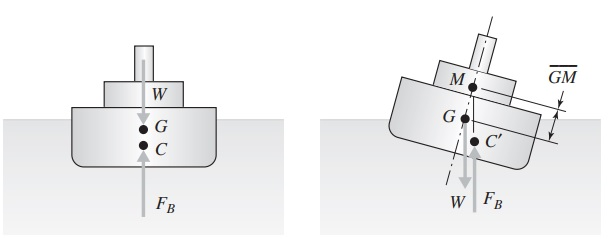
\includegraphics[width = .6\linewidth]{U2-estabilidad3.jpg}
	\caption{Sección transversal cuerpo en flotación}
	\label{fig:sec-transv}
\end{figure}
\begin{multicols}{2}
	\begin{tabular}{c}
		El valor de $\widehat{GM}$ se puede calcular como\\
		$\widehat{GM}=\dfrac{I_{o}}{V_{desplazado}}-\widehat{CG}$\\
	\end{tabular}
	\begin{tabular}{c}
		El valor del momento restaurador:\\
		$C=\gamma~ \Delta \theta~ I_{yy}$\\
	\end{tabular}
\end{multicols}

\subsection{Equilibrio relativo}

\subsubsection{Aceleración lineal uniforme}	
El fluido se encuentra en reposo con relación a un marco de referencia acelerado en \emph{x} e \emph{y}. Recordando la ecuación \ref{eq:variacion-de-presion}, esta se simplifica a:
\begin{equation}
	dp = - \rho a_{x} dx - \rho(g + a_{z}) dz
\end{equation} 

Integrando entre los puntos 1 y 2 tenemos:

\begin{equation}
	p_{2}- p_{1} = - \rho a_{x}(x_{2}-x_{1}) - \rho(g + a_{z}) (z_{2}-z_{1})
\end{equation}
\begin{figure}[h]
	\centering
	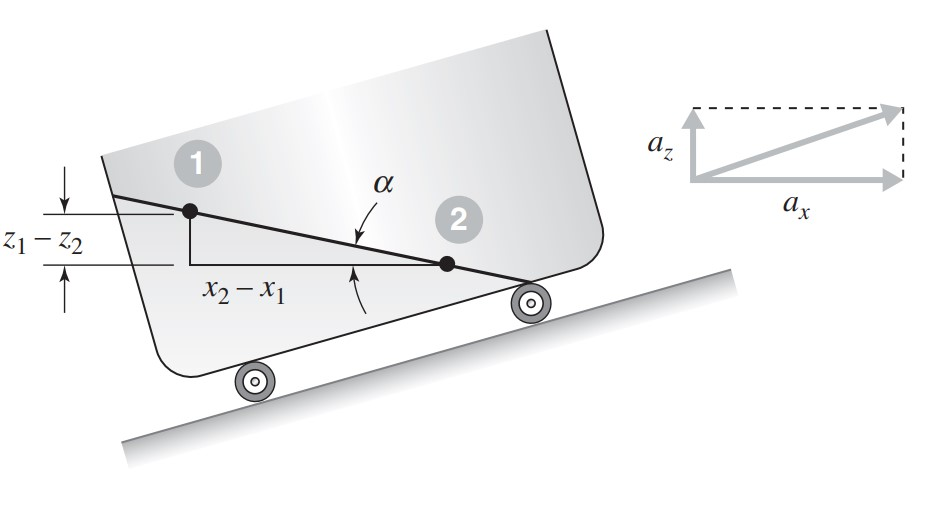
\includegraphics[width = .5\linewidth]{U2-aceleracion-lineal}
	\caption{Depósito linealmente acelerado}
\end{figure}

Si los puntos 1 y 2 se encuentran a la misma presión entonces:
\begin{equation}
	\dfrac{z_{1}-z_{2}}{x_{2}-x_{1}} = \tan \alpha = \dfrac{a_{x}}{g-a_{z}}
\end{equation}
\\
\subsubsection{Rotacion uniforme alrededor de un eje vertical}

La ecuacion diferencial de presion:
\begin{equation}
	dp = \rho r \omega^{2} dr - \rho g dz
\end{equation}
Si elegimos el centro de coordenadas en el vértice del paraboloide e integramos la ecuación.
\begin{equation}
	p -p_{0} = \dfrac{\rho \omega^{2} }{2} r^{2} - \rho g z
\end{equation}
\begin{figure}[h]
	\centering
	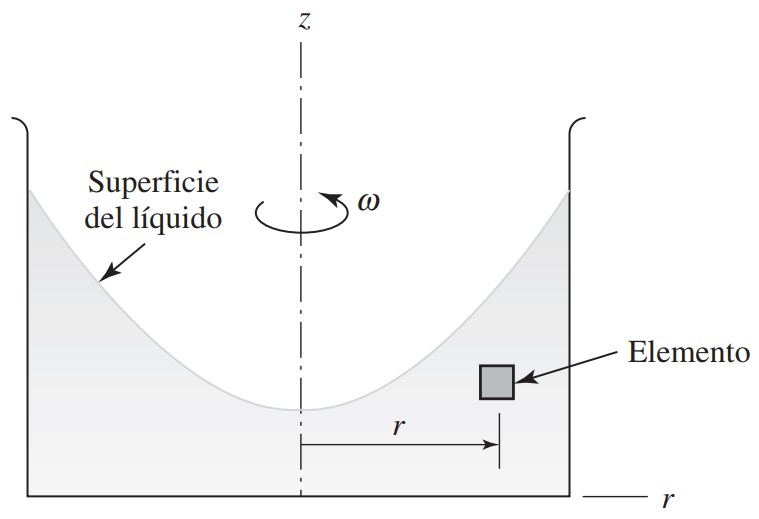
\includegraphics[width = .4\linewidth]{U2-rotacion-uniforme}
	\caption{Depósito sometido a rotación}
\end{figure}
Si los dos puntos considerados se encuentran a la misma presión como la superficie libre entonces $p - p_{0} = 0$ y nos queda una ecuación de una parábola que corta el origen:

\begin{equation}
	z = \dfrac{\omega^{2} r^{2} }{2 g}
\end{equation}

El origen de coordenadas se puede encontrar igualando el volumen del fluido en reposo y cuando se encuentra en rotación uniforme.
	%\section{Teoría del flujo unidimensional}


\subsection{Sistema y volumen de control}

\subsubsection{Sistema de control}
Un sistema de control se refiere a una masa fija (infinitesimal o finita) definida y se distingue de todas las demás. Las fronteras del sistema forman una superficie cerrada. Esta superficie puede variar en el tiempo de tal manera que mantenga la misma masa durante los cambios. Es decir $dm/dt = 0$.
En el enfoque \emph{Lagrangiano} en el cual el estudio se centra en el movimiento de partículas individuales, el movimiento se observa como una función del tiempo. Es decir se "sigue" a la partícula, como en el estudio de sólidos. En este caso se utiliza un sistema de control, ya que la masa de la partícula o solido se mantiene constante

\subsubsection{Volumen de control}
En el enfoque \emph{Euleriano} se mantiene fija la coordenada espacial y así se pueden observar las velocidades de las partículas móviles al pasar por esta posición en cualquier instante. Entonces, las propiedades del flujo son funciones del espacio y el tiempo.
Este tipo de enfoque se puede estudiar a través de un volumen de control o punto fijo, en el cual el flujo pasa a traces de este.

%%%%%%%%%%%%%%%%%%%%%%%%%%%%%%%%%%%%%%%%%%%%%%%%%%%%%%
\subsection{Linea y tubo de corriente}

\subsubsection{Linea de trayectoria}
Es el lugar geométrico de los puntos recorridos por una partícula determinada cuando se desplaza en un campo de flujo.

\subsubsection{Linea de corriente}
Es una línea continua que representa el flujo y ésta posee la propiedad de que el vector velocidad de cada partícula es tangente a la línea de corriente. La ecuacion que representa el vector: $ \overline{v} x d\overline{r} = 0$

\begin{figure}[h]
	\centering
	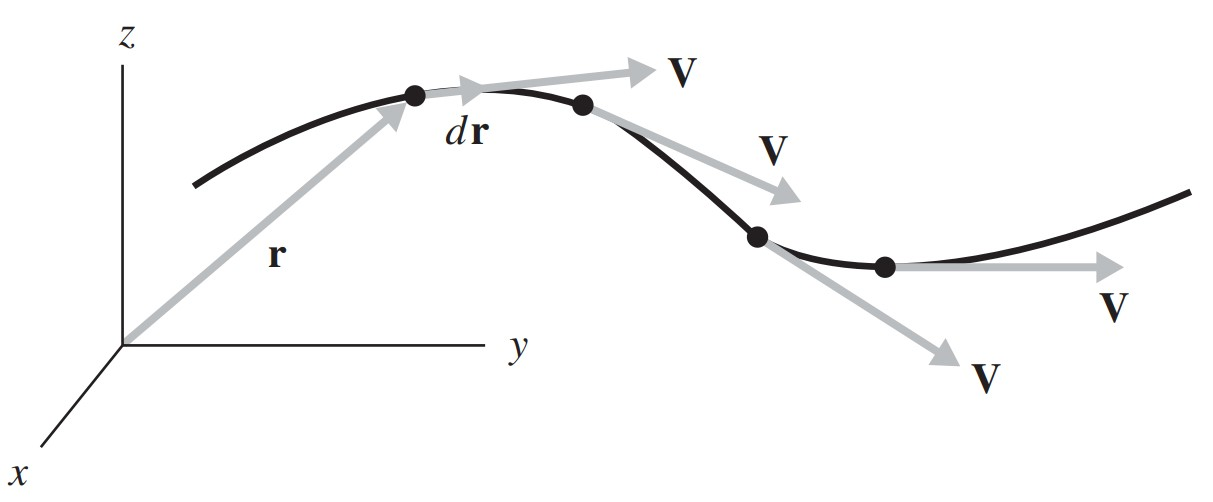
\includegraphics[width = .5\linewidth]{U3-linea-corriente}
	\caption{Linea de corriente en un campo de flujo}
\end{figure}

En un flujo \emph{permanente} la trayectoria de una partícula es una linea de corriente. Pero en un flujo no permanente donde el vector velocidad cambia con el tiempo, haciendo que la partícula siga diferentes lineas de corrientes de tal manera que la trayectoria de esta no puede parecerse a ninguna linea de corriente.

\subsubsection{Tubo de corriente}
Un tubo de corriente está constituido por una región parcial del flujo delimitada por una familia de lineas de corriente. No existe flujo a través de las paredes ya que el vector velocidad no tiene componete perpendicular a la superficie del tubo ya que siempre es tangente a la linea de corriente.

%%%%%%%%%%%%%%%%%%%%%%%%%%%%%%%%%%%%%%%%%%%%%%%%%%%%%%%%%%%%%%%
\subsection{Tipos de flujo}
\subsubsection{Flujo permanente}
Ocurre cuando las condiciones en cualquier punto del fluido no cambian con el tiempo es decir:

\begin{tabular}{r c l}
	$\dfrac{\delta v}{\delta t} = 0$ & $\dfrac{\delta p}{\delta t}$ & $ \dfrac{\delta \rho}{\delta t}$
\end{tabular}

Esto no significa que la velocidad no varíe de un punto.

\subsubsection{Flujo en una, dos y tres dimensiones}

\subsubsection{Flujo laminar y turbulento}
En un \textbf{flujo laminar} las partículas se mueven a lo largo de trayectorias suaves en láminas o capas, con una capa deslizándose suavemente sobre otra adyacente. El flujo laminar está gobernado por la ley de viscosidad de Newton, la cual relaciona el esfuerzo cortante con la tasa de deformación angular. En situaciones de baja viscosidad, alta velocidad o grandes caudales, este flujo no es estable y se rompe en flujo turbulento.\\

En un \textbf{flujo turbulento} los movimientos del fluido varían irregularmente. Las partículas se mueven en trayectorias arremolinadas causando un intercambio de momentum. La turbulencia causa mayores esfuerzos cortantes y pérdidas.\\

Si un flujo es laminar o turbulento depende de tres parámetros físicos que combinados forman el número de \textbf{Reynolds} y nos permite determinar el régimen de flujo:\\

\begin{tabular}{c c}
		\begin{minipage}[t]{.45\textwidth}
			\flushright 
			\vspace{.05cm}
			$Re= \dfrac{V L}{\nu}$
		\end{minipage}
		&
		\begin{minipage}[t]{.45\textwidth}
			\flushleft
			V velocidad\\
			L Longitud\\
			$\nu$ viscosidad cinemática
		\end{minipage}
\end{tabular}

\subsubsection{Flujos viscosos e inviscidos}
\subsubsection{Flujo compresible e incompresible}
		



%%%%%%%%%%%%%%%%%%%%%%%%%%%%%%%%%%%%%%%%%%%%%%%%%%%%%%%%%%%%

\end{document}